\documentclass[paper=a4, fontsize=11pt]{scrartcl}
\usepackage[T1]{fontenc}
\usepackage{fourier}
\usepackage[numbers]{natbib}
\usepackage[english]{babel}	
% English language/hyphenation
\usepackage[protrusion=true,expansion=true]{microtype}	
\usepackage{amsmath,amsfonts,amsthm} % Math packages
\usepackage[pdftex]{graphicx}	
\usepackage{url}
\usepackage[
backend=biber,
style=numeric,
sorting=ynt
]{biblatex}
\addbibresource{refs.bib}
\usepackage{enumitem}

\newlength\tindent
\setlength{\tindent}{\parindent}
\setlength{\parindent}{0pt}
\renewcommand{\indent}{\hspace*{\tindent}}

%%% Custom sectioning
\usepackage{sectsty}
\allsectionsfont{\centering \normalfont\scshape}


%%% Custom headers/footers (fancyhdr package)
\usepackage{fancyhdr}
\pagestyle{fancyplain}
\fancyhead{}											% No page header
\fancyfoot[L]{}											% Empty 
\fancyfoot[C]{}											% Empty
\fancyfoot[R]{\thepage}									% Pagenumbering
\renewcommand{\headrulewidth}{0pt}			% Remove header underlines
\renewcommand{\footrulewidth}{0pt}				% Remove footer underlines
\setlength{\headheight}{13.6pt}


%%% Equation and float numbering
\numberwithin{equation}{section}		% Equationnumbering: section.eq#
\numberwithin{figure}{section}			% Figurenumbering: section.fig#
\numberwithin{table}{section}				% Tablenumbering: section.tab#


%%% Maketitle metadata
\newcommand{\horrule}[1]{\rule{\linewidth}{#1}} 	% Horizontal rule

\title{
		%\vspace{-1in} 	
		\usefont{OT1}{bch}{b}{n}
		\normalfont \normalsize \textsc{The University of Texas at Austin} \\ [25pt]
		\horrule{0.5pt} \\[0.4cm]
		\huge Statistical Modeling II Project \\
		\horrule{2pt} \\[0.5cm]
}
\author{
		\normalfont 								\normalsize
        Juliette Franqueville\\[-3pt]		\normalsize
        \today
}
\date{}


%%% Begin document
\begin{document}
\maketitle
\newpage
\section{Introduction}

The COVID-19 pandemic resulted in stay-at-home orders across the world. As a result, people spent more time at home and in outdoor areas and less time commuting to work or restaurants. This report explores the relationship between the changes in mobility patterns of the general population and the number of incidents reported by fire departments in the United States in 2020. Several studies have already explored the effect of COVID-19 on fire incidents. For example, Suzuki and Manzello \cite{fire_paper} analyzed the effect of stay-at-home orders on cooking fires in major cities. Koester and Greatbatch \cite{koester2020comparing} investigated the impact of the onset of the pandemic on fire and search and rescue incident frequency. This report utilizes NFORS \cite{nfors} analytics data provided by the International Public Safety Data Institute and 2020 Google Mobility data \cite{google}. The names of the fire departments were hidden for anonymity. 

\section{Data Formatting}
The raw datasets were formatted to obtain weekly averages for number of incident percentage change from baseline for 2020 for each fire department in NFORS and 2020 weekly average Google mobility data corresponding to the county of each NFORS department.\\


The Google data columns of interest were date,  FIPS code (which corresponds to unique county) and percentage change from baseline for workplace, retail, parks, and grocery/pharmacy mobility. First, the Google mobility data were grouped by FIPS codes.  The data with FIPS codes corresponding to those of the counties of the fire departments in the NFORS data were kept.\\



The Google mobility data is reported as a percentage change from baseline. The baseline used is the median value for each day of the weeks over the January 3rd - February 6th 2020 period. To get a weekly average, a 7-day rolling average was used and the value for all Mondays was reported as the weekly average. \\

In the NFORS data, the data of interest were date, fire department, and number of incidents reported for each date. For each fire department, gaps in data (where more than two consecutive days had zero incidents, which is very unlikely) were removed. Then, outliers were removed by fitting a negative binomial distribution to the incident counts of each department using moment matching and removing points outside the 95 \% confidence interval.\\


An incident baseline was calculated from the 2019 NFORS data and applied to the 2020 data. The baseline was calculated by taking the median of the number of incidents per day of the week per month for each department. Accounting for month as well as day of the week ensured that the seasonality in fire incidents was accounted for. Then, the percentage change for each day in 2020 was calculated from this baseline. Note that some departments were missing significant amounts of data and did not allow for calculating a baseline for each month and each day of the week in 2019. For missing baseline data points, the corresponding changes from baseline in 2020 could not be calculated.  Some department had no data for 2019, so they were not used in the analysis, As with the Google data, a weekly average for incident percentage change form baseline for each department was calculated. \\

 The resulting data format was an $X_i \in \mathbb{R}^{n_i \times p}$ matrix for each department, where $p$ is the number of mobility types (workplace, retails, etc), $i$ is the department, and $n_i$ is the number of weekly averages for each department. Note that ideally, each department would have $n_i = 52$ because there are 52 weeks in a year, but the Google mobility data only begins in February 2020 and some departments had missing data. Each department also had a $y_i \in \mathbb{R}^{n_i}$ vector of incident percentage change from baseline corresponding to the $X_i$ matrices. Additionally, each department had a $t_i \in \mathbb{R}^{n_i}$ vector containing the day of the year that the observations are for (days all correspond to Mondays because the weekly averages were evaluated on Mondays).


\section{Data Exploration}
As expected, the various mobility types were highly correlated. Figure \ref{corr_mat} shows the correlation matrix for the mobility types.


\begin{figure}[h]
\caption{Example of a parametric plot ($\sin (x), \cos(x), x$)}
\centering
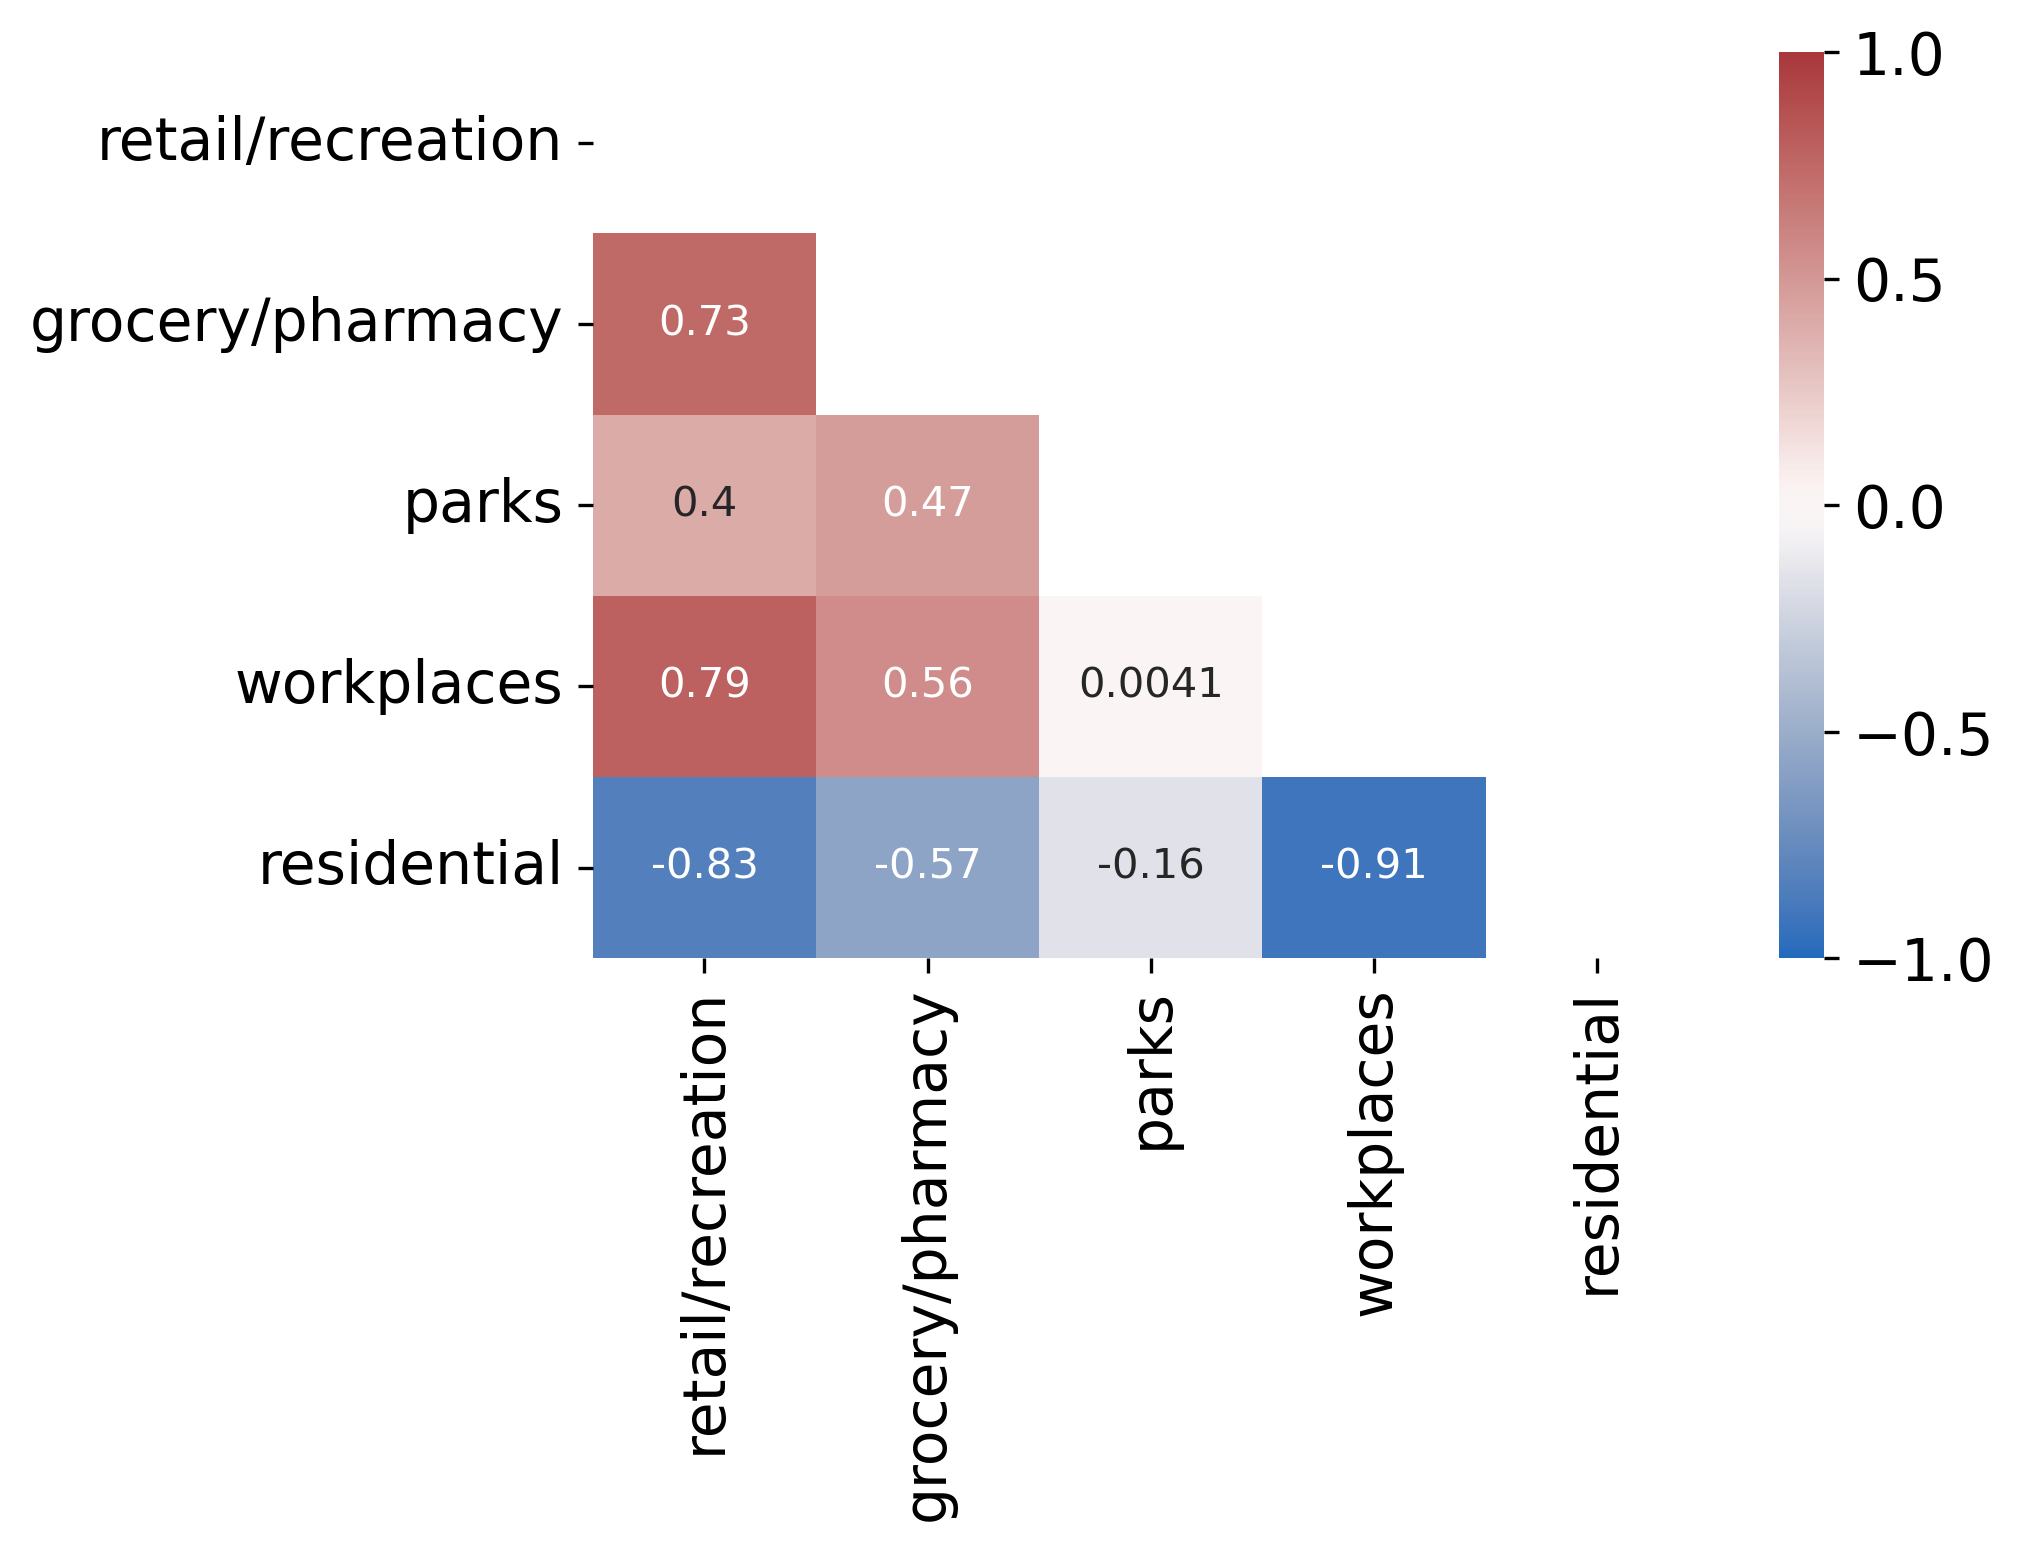
\includegraphics[width=0.5\textwidth]{corr.png}
\end{figure}



\section{Model}
\section{Results}





\printbibliography

\end{document}